\documentclass[preprint,12pt]{elsarticle}

\usepackage{amssymb}


\journal{Proceedings of the Royal Society B}

%%%%%%%%%%%%%%% my adding usepackages
%amsmath package provides an environment subequations
\usepackage{amsmath}

\usepackage{hyperref}

\usepackage{graphicx}
\usepackage{color} 

%\usepackage{showframe}

% comments
\usepackage{ulem}
\definecolor{purple}{rgb}{0.459,0.109,0.538}
\def\tb#1#2{\sout{#1} \textcolor{purple}{#2}}
\def\tbc#1{\textcolor{purple}{[#1]}}
\definecolor{blue}{rgb}{0.324,0.609,0.708}
\def\al#1#2{\sout{#1} \textcolor{blue}{#2}} 
\def\alc#1{\textcolor{blue}{[#1]}} 

\begin{document}

\begin{frontmatter}

%% Title, authors and addresses

%% use the tnoteref command within \title for footnotes;
%% use the tnotetext command for the associated footnote;
%% use the fnref command within \author or \address for footnotes;
%% use the fntext command for the associated footnote;
%% use the corref command within \author for corresponding author footnotes;
%% use the cortext command for the associated footnote;
%% use the ead command for the email address,
%% and the form \ead[url] for the home page:
%%
%% \title{Title\tnoteref{label1}}
%% \tnotetext[label1]{}
%% \author{Name\corref{cor1}\fnref{label2}}
%% \ead{email address}
%% \ead[url]{home page}
%% \fntext[label2]{}
%% \cortext[cor1]{}
%% \address{Address\fnref{label3}}
%% \fntext[label3]{}

%Title of paper
\title{Modeling the effects of vaccination on influenza transmission and evolution}

%% use optional labels to link authors explicitly to addresses:
%% \author[label1,label2]{<author name>}
%% \address[label1]{<address>}
%% \address[label2]{<address>}

\author{Alvason Zhenhua Li}
\ead{alvali@fredhutch.org}

\author{Trevor Bedford}
\ead{tbedford@fredhutch.org}


\address{Vaccine and Infectious Disease Division, Fred Hutchinson Cancer Research Center, Seattle, WA 98109, USA}


\begin{abstract}
Influenza viruses continually evolve to escape the human population immune response.
New antigenic variants have a transmission advantage over older strains and so spread to take over the influenza virus population.
Previous work has sought to model the join epidemiological and evolutionary process in which competition between strains plays out.
By assuming a linear strain space, many of the basic dynamics of influenza transmission and evolution can captured.
These models show a pattern of limited standing antigenic diversity, but rapid strain turnover coincident with observed dynamics.
Here, we extend previous models to incorporate the effects of vaccination on influenza transmission and evolution.
We examine varying vaccination coverage, vaccine strain choice and vaccination age cohort.
We find that increasing vaccination coverage results in decreased disease incidence and slower rates of antigenic evolution.
Interestingly, we find that vaccinating with antigenically leading strains, not matched to circulating viruses, results in better overall protection.
We also find that the same vaccine coverage applied to infants, before first influenza infection, rather than equally across the population, results in slower virus evolution and better overall protection.
\end{abstract}

\begin{keyword}
%% keywords here, in the form: keyword \sep keyword
Influenza\sep Vaccination\sep Immunity\sep Mutation
\end{keyword}

\end{frontmatter}

%% main text
\section{Introduction}
Vaccination is one of the major medical advances in fighting various virus in recent centuries.
Currently, influenza vaccination is a powerful tool in the global-health control arsenal, and allows for the mass prevention of infection.
Various elements of mathematics are used throughout the vaccine development process.
In this paper, we focus on the use of mathematics in influenza virus drift, understanding the impact of vaccination at the many-strain antigenic evolution. 

\section{Model}
Mathematically, based on the many-strain SIR epidemiological model (Gog and Grenfell 2002), which specifies the dynamics of large number of antigenic types with cross-immunity interaction, and introduced the general vaccination strategy composing infants (a proportion \(\phi_{new}\) of all children are assumed to be immunized) and the random vaccination of individuals in the population (at rate \(\phi_{pulse}\), although this vaccination will only affect those that are currently susceptible).
We are able to developed a many-strain SIRV epidemiological model as the following:

\begin{align}
  \label{eq:S}
  \frac{\partial S_i(x,t)}{\partial t} = \mu N(1-\phi_{new}(t)\sum_{y=0}^{n} \sigma(x,y)) - \mu S_i(x,t) - \phi_{pulse}(t)\sum_{y=0}^{n} S_i(y,t)\sigma(x,y) 
  \nonumber\\
  - \beta S_i(x,t)\sum_{y=0}^{n} I_i(y,t)\sigma(x,y)
\end{align}

\begin{equation}
  \label{eq:I}
  \frac{\partial I_i(x,t)}{\partial t} = \beta S_i(x,t) I_i(x,t) - \mu I_i(x,t) - \nu I_i(x,t) + m \frac{\partial^2I_i(x,t)}{\partial x^2}
\end{equation}

\begin{equation}
  \label{eq:R}
  \frac{\partial R_i(x,t)}{\partial t} = \nu I_i(x,t) - \mu R_i(x,t) - \beta S_i(x,t) [I_i(x,t) - \sum_{y=0}^{n} I_i(y,t)\sigma(x,y)]
\end{equation}

\begin{equation}
  \label{eq:V}
  \frac{\partial V_i(x,t)}{\partial t} = \mu N \phi_{new}(t)\sum_{y=0}^{n} \sigma(x,y) + \phi_{pulse}(t)\sum_{y=0}^{n} S_i(y,t)\sigma(x,y) - \mu V_i(x,t)
\end{equation}

where the cross-immunity kernel \(\sigma(x,y)\) is an inverse form of the Monod equation:
\begin{equation}
  \label{eq:Immunity}
  \sigma(x,y) = 1 - \frac{\vert {\frac{x -y}{r}} \vert}{1 + \vert {\frac{x -y}{r}} \vert}
\end{equation}

\begin{figure}
  \centering
  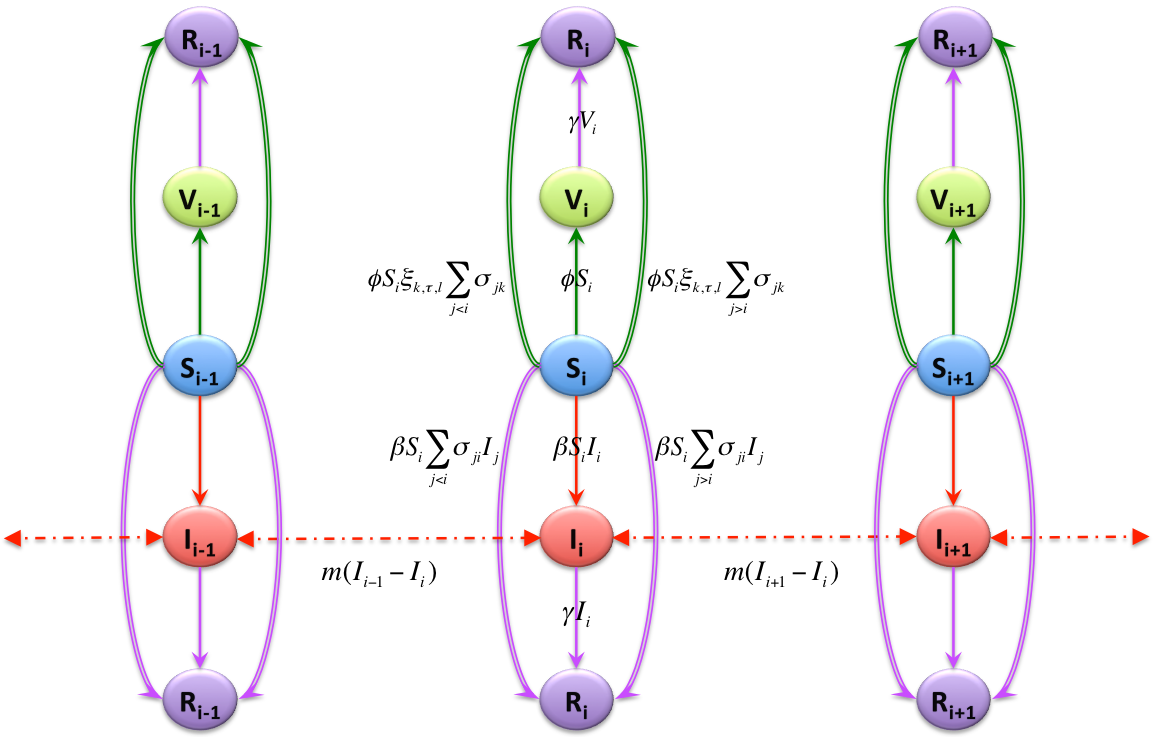
\includegraphics[width=6in,height=3in]{figures/Diagram}
  \caption{Schematic diagram of the many-stain SIRV model.
  The solid straight arrows indicate the classic single-strain SIRV relationship.
  The double-line arrows indicate the cross-immunity relationship with nearby strains.
  The dashed double-arrows indicate the mutation to nearby strains. For simplification, both the birth and death rate \(\mu\) are ignored in this diagram.}
\label{fig:Diagram}
\end{figure}

\begin{figure}
  \centering
  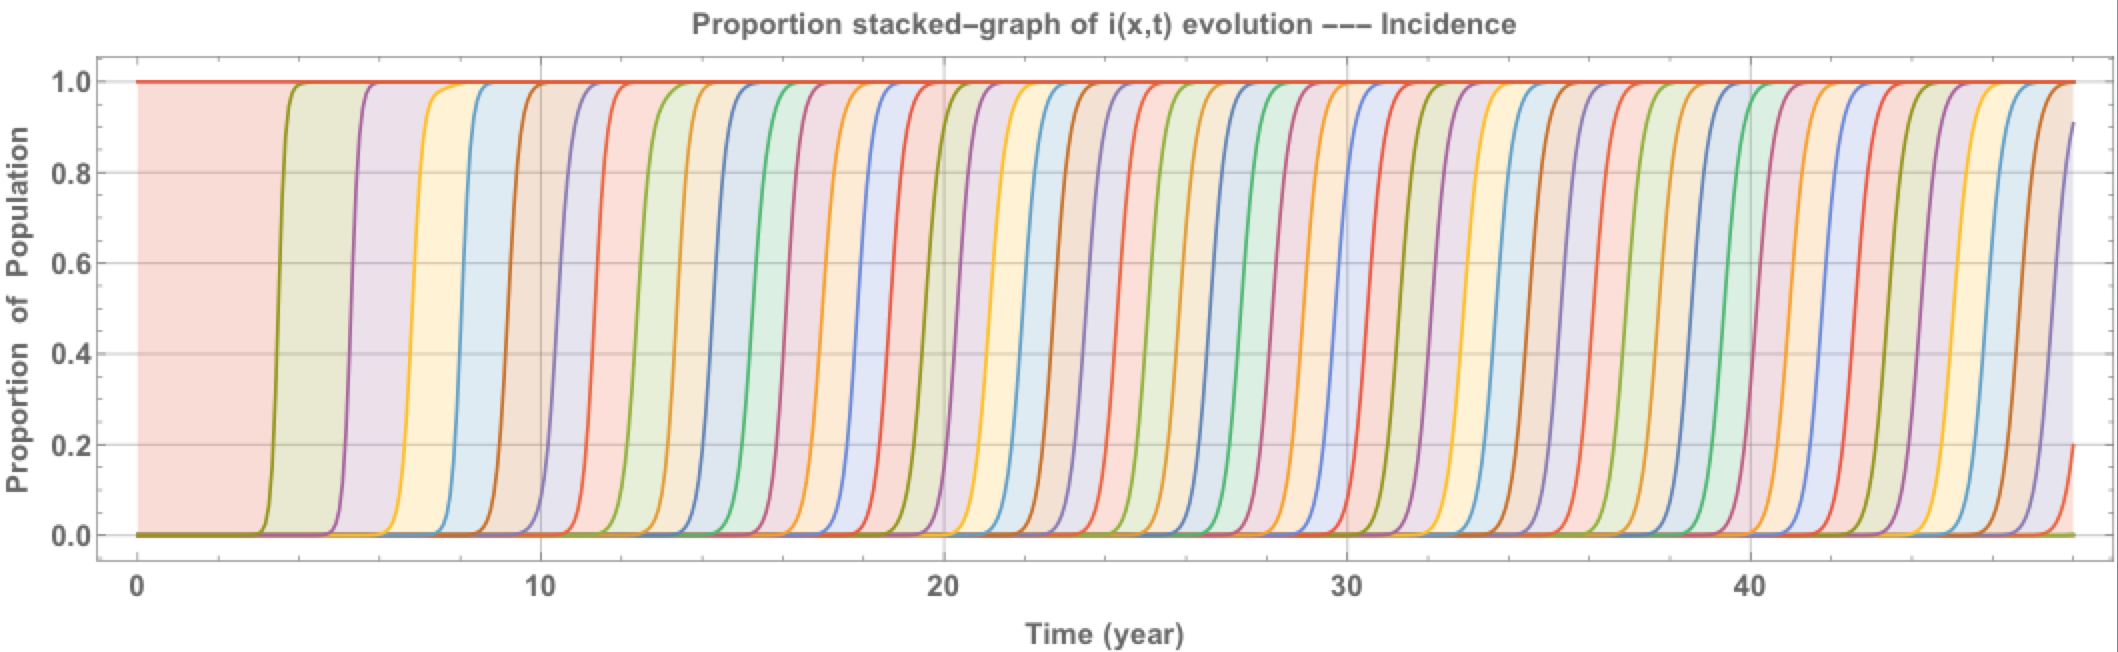
\includegraphics[width=6in,height=3in]{figures/Proportion}
  \caption{Proportion stacked graph indicated the building up process of steady traveling wave of influenza drift.
  Initial single-strain-equilibrium-state is propagating into many-strain-equilibrium-state.}
\label{fig:Proportion}
\end{figure}


\section{Results}

\begin{figure}
  \centering
  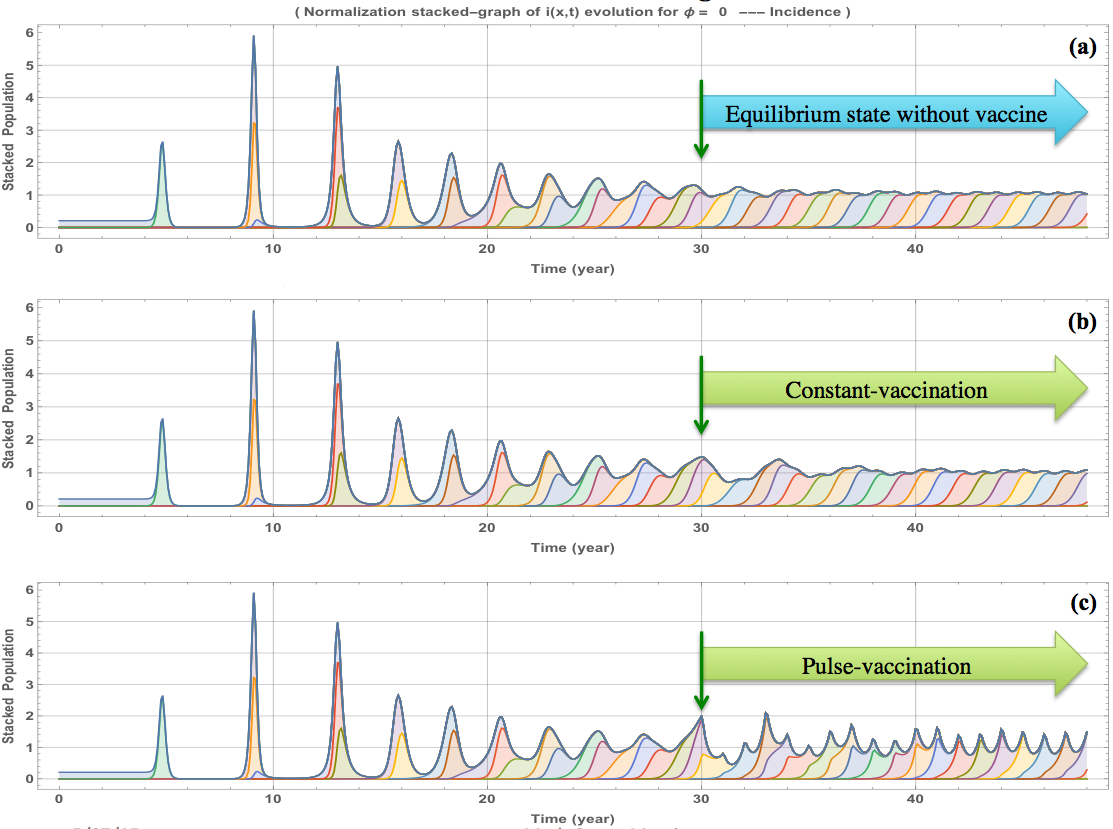
\includegraphics[width=6in,height=4in]{figures/UnderVaccination}
  \caption{Comparison of incidence rate between non-vaccination and under-vaccination.
  (a) is a stain evolutionary map without vaccination (vaccination rate \(\phi\) = 0), in which a single-strain-equilibrium-state is evolving into many-strain-equilibrium-state in a half century time frame. 
  (b) is the strain evolutionary map with 20 years vaccination: at the beginning 30 years, a single-strain-equilibrium-state is approaching into many-strain-equilibrium-state, however, starting from the 30th year, an annual vaccination strategy (vaccination rate \(\phi\) = 0.039 ) is applied. 
  After 20 years of vaccination pressure, the evolution is evolving and approaching into vaccination-equilibrium state.}
\label{fig:UnderVaccination}
\end{figure}


\section{Analysis}
\begin{figure}
  \centering
  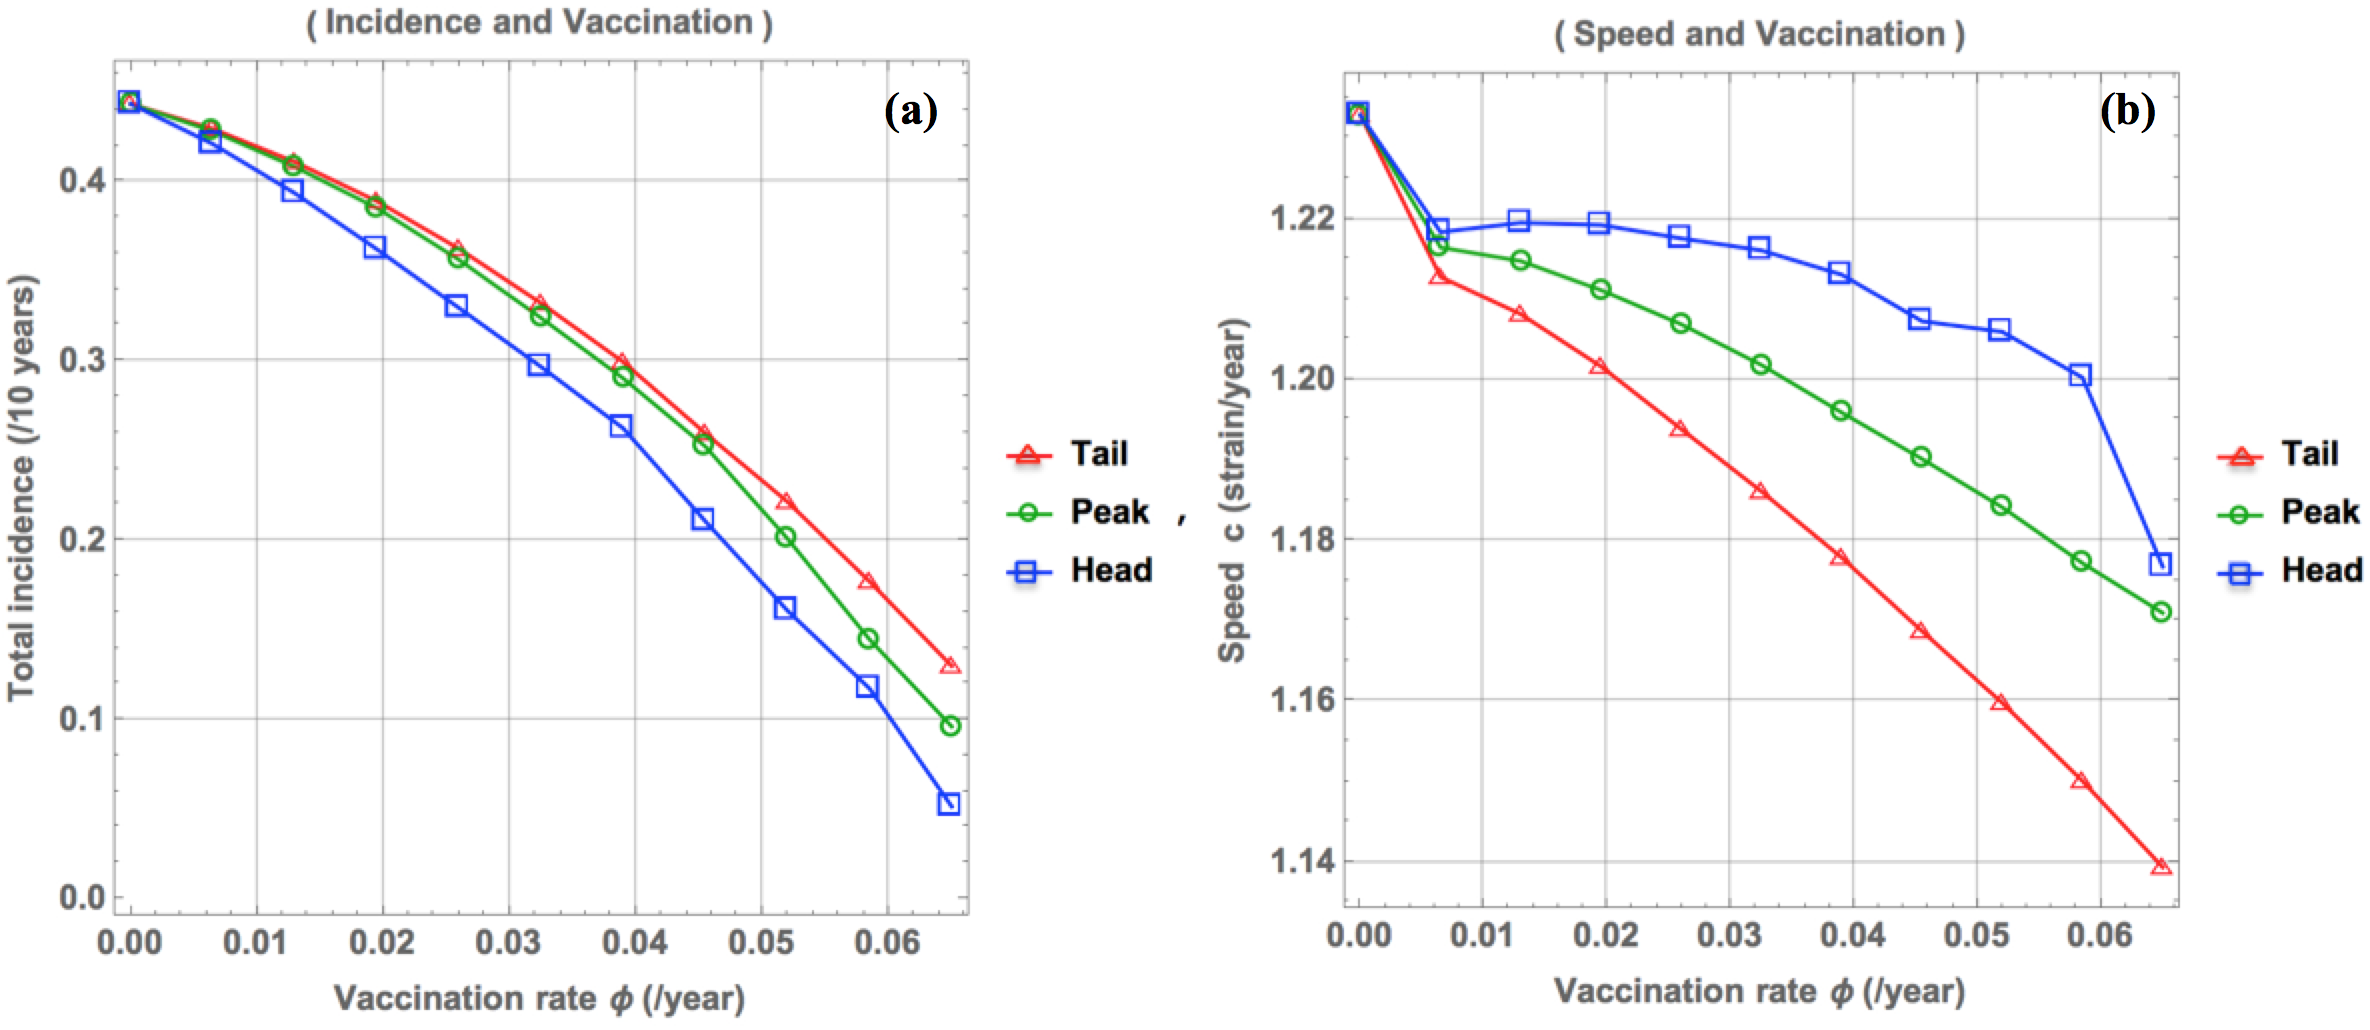
\includegraphics[width=6in,height=2.75in]{figures/Veffect}
  \caption{Effects of vaccination on disease incidence and speed of antigenic drift. tytttyytytty
  (a) Incidence or attack rate is measured as the average proportion of the population infected yearly.
  \tbc{Change $y$-axis label to ``Attack rate (/year)'' and divide these numbers by 10. People are more used to seeing attack rate per year than attack rate per 10 years.}
  (b) Antigenic drift rate is measured as the average difference between the mean antigenic phenotype at time \(t\) and the mean antigenic phenotype at time \(t+1\).
  Vaccination rate \(\phi\) is measured in terms of the proportion of the population vaccinated yearly.
  \tbc{Remove plot labels ``(Incidence and Vaccination)'' and ``(Speed and Vaccination)''. Can see this from the $y$-axes.}
  }
  \label{fig:Veffect}
\end{figure}



\begin{figure}
  \centering
  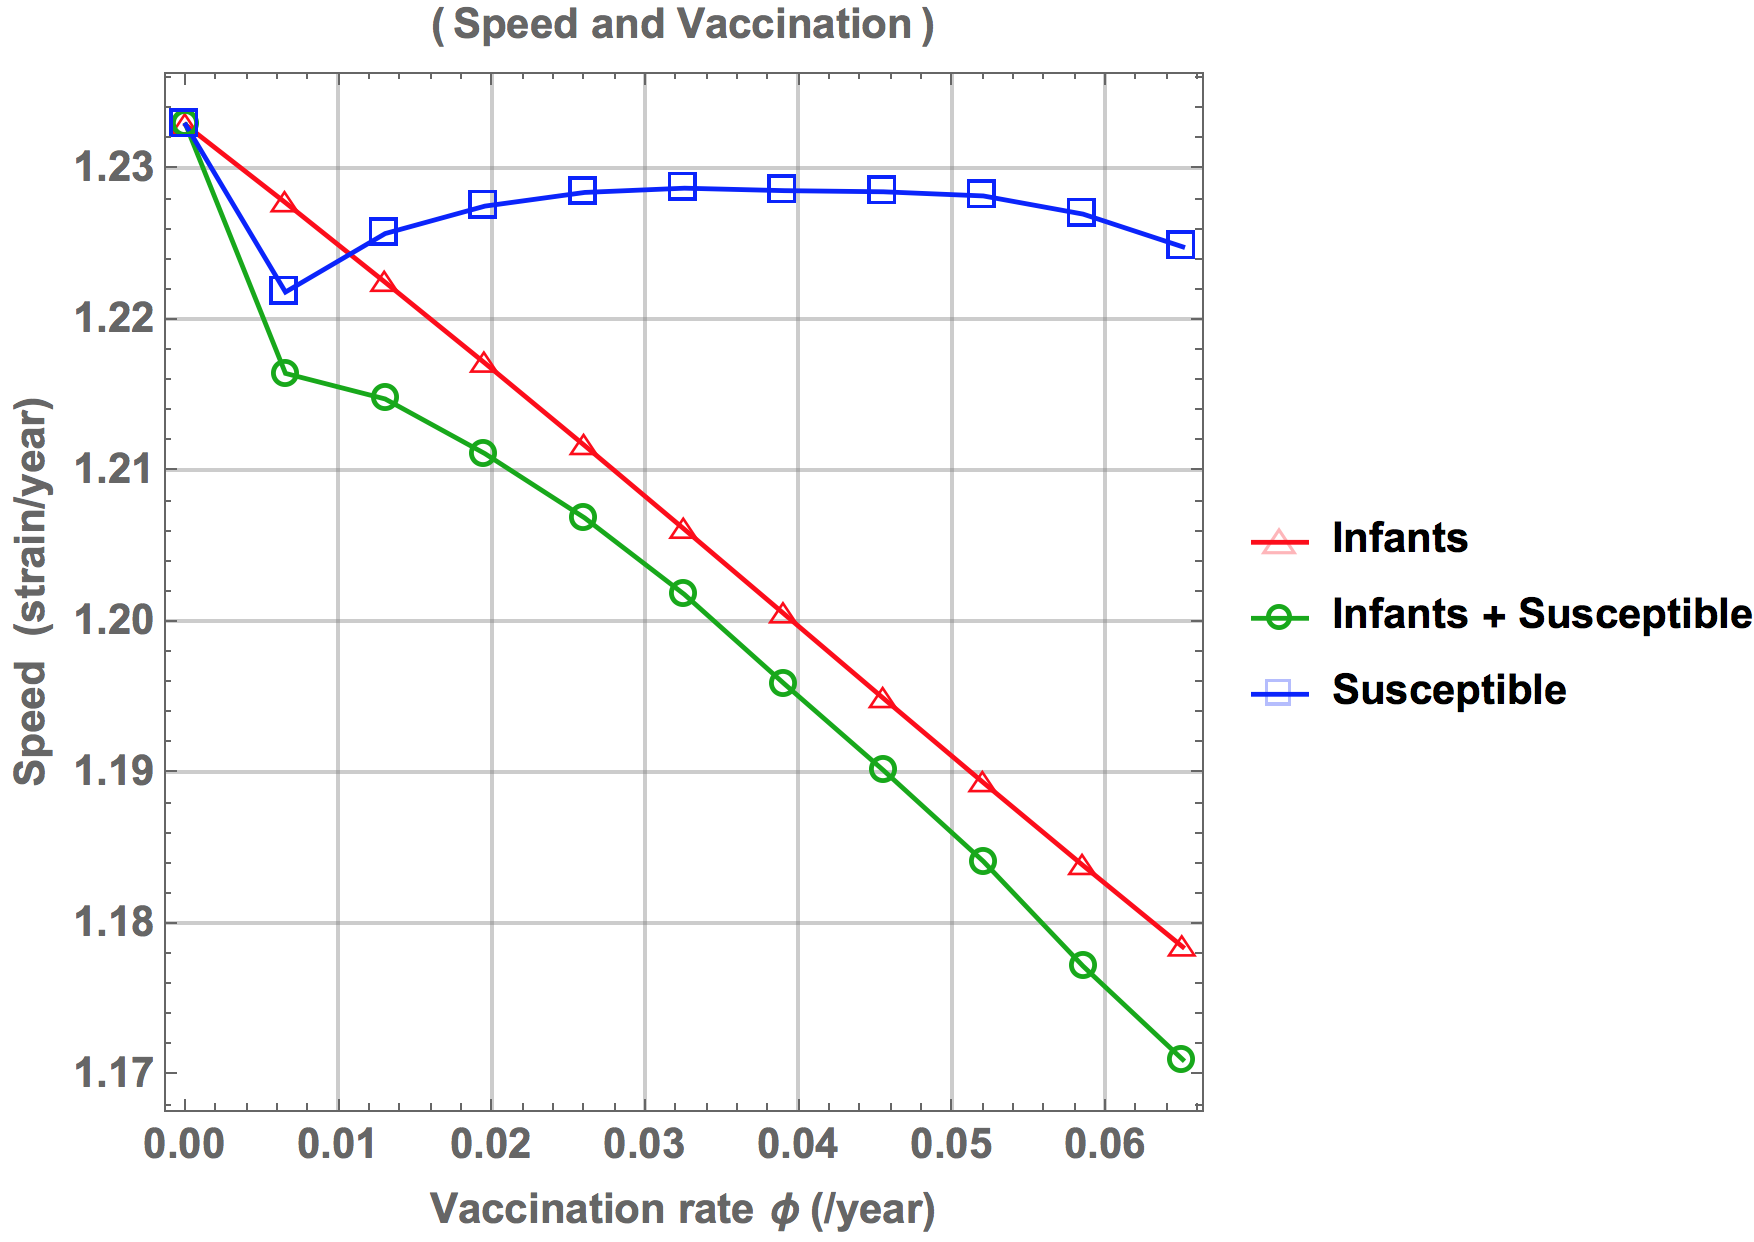
\includegraphics[width=6in,height=4in]{figures/NewbornS}
  \caption{Contribution from two vaccination strategies.
  The triangle-marker red line is the strain evolutionary speed as a function of infant-vaccination-rate only, while the rectangle-marker blue line is the strain evolutionary speed as a function of susceptible-vaccination-rate only.
  The circle-marker green line is the composition of both vaccination strategy.}
  \label{fig:NewbornS}
\end{figure}

Test edit.


\section{Conclusion}
In conclusion, exact.

%% The Appendices part is started with the command \appendix;
%% appendix sections are then done as normal sections
%% \appendix

%% \section{}
%% \label{}

%% References
%%
%% Following citation commands can be used in the body text:
%% Usage of \cite is as follows:
%%   \cite{key}         ==>>  [#]
%%   \cite[chap. 2]{key} ==>> [#, chap. 2]
%%

%% References with bibTeX database:

\bibliographystyle{elsarticle-num} %with article and chapter titles,

%\bibliographystyle{model1a-num-names} %without article and chapter titles


% Create the reference section using BibTeX:
\bibliography{ReferenceMorse}

%% Authors are advised to submit their bibtex database files. They are
%% requested to list a bibtex style file in the manuscript if they do
%% not want to use elsarticle-num.bst.

%% References without bibTeX database:

% \begin{thebibliography}{00}

%% \bibitem must have the following form:
%%   \bibitem{key}...
%%

% \bibitem{}

\end{document}
